\chapter{実装}
本章では,ADLoggerシステムの実装について述べる.
はじめに実装環境について述べ,ついでタスク別時間記録モジュール,必要時間予測モジュールについて説明する.

\section{実装環境}
本節では,本システムにおける実装環境について説明する.本システムはiPhoneアプリケーションであり,実装言語にはSwiftを使用している.
サーバサイド兼データベースには,MBaaS (Mobile Backend as a Service)であるBack4App~\cite{back4app}を利用している.

\section{クライアント側実装}
クライアントはiPhoneアプリケーションであり,Swiftによって実装した.
タスク別時間記録モジュール,必要時間予測モジュールについて説明する.

\subsection{タスク別時間記録モジュール}
本節ではタスク別時間記録モジュールについて説明する.
タスク別時間記録モジュールはユーザが行動したタスク及び時間を記録するモジュールである.
メイン画面のUIButton``TIMER"を押すと,ストップウォッチ画面に遷移する.(図~\ref{fig:stopwatch}参照)
UIButton``START"を押すとUIButtonが``STOP"に書き換えられた後,
上段に配置したUILabel``00:00:00"から “hh:mm:ss”の書式で書き換えられ経過時間が表示される.

\begin{figure}[ht]
\begin{center}
\begin{tabular}{c}

	\begin{minipage}[b]{0.5\linewidth}
	\begin{center}
		\fbox{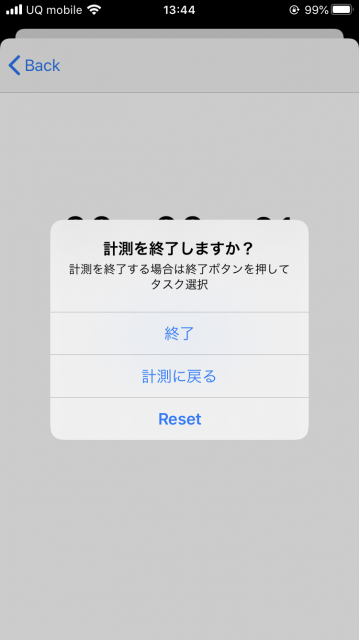
\includegraphics[width=5cm]{images/6/salert.png}}
		\caption{計測に関する選択}
		\label{fig:salert}
	\end{center}
  	\end{minipage}
	
	\begin{minipage}[b]{0.5\linewidth}
	\begin{center}
		\fbox{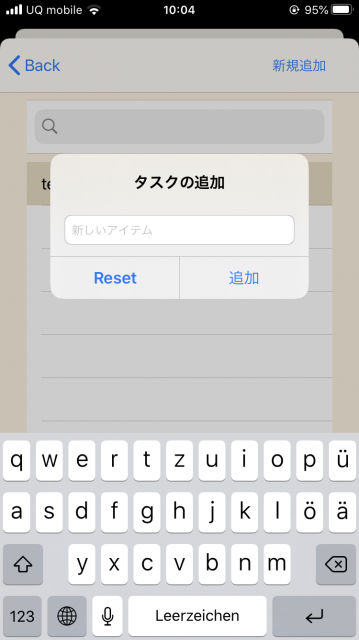
\includegraphics[width=5cm]{images/6/newtask.png}}
		\caption{新規追加}
		\label{fig:newtask}
	\end{center}
  	\end{minipage}
	
	\\
	
	\begin{minipage}[b]{0.5\linewidth}
	\begin{center}
		\fbox{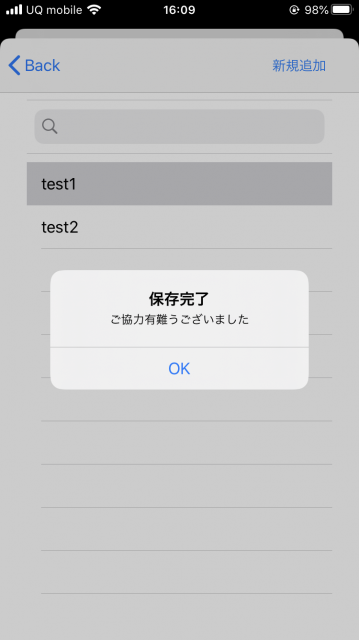
\includegraphics[width=5cm]{images/6/saved.png}}
		\caption{保存完了}
		\label{fig:saved}
	\end{center}
  	\end{minipage}
	
	\begin{minipage}[b]{0.5\linewidth}
	\begin{center}
		\fbox{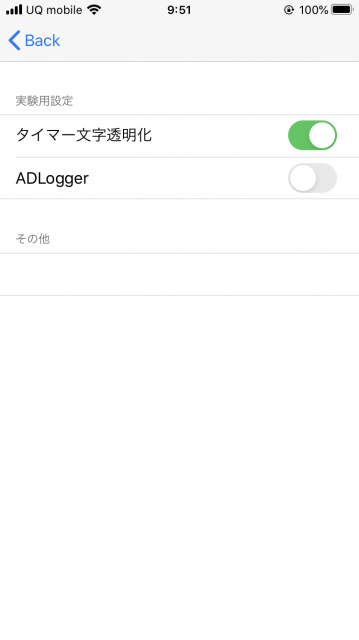
\includegraphics[width=5cm]{images/6/setting.png}}
		\caption{設定画面}
		\label{fig:setting}
	\end{center}
  	\end{minipage}

\end{tabular}
\end{center}
\end{figure}

\begin{figure}[ht]
\begin{center}
\begin{tabular}{c}

	\begin{minipage}[b]{0.5\linewidth}
	\begin{center}
		\fbox{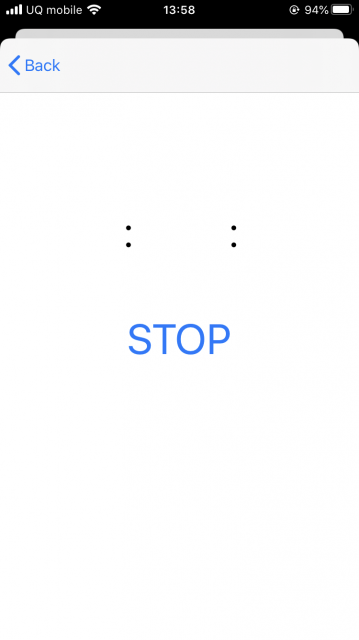
\includegraphics[width=5cm]{images/6/hidden.png}}
		\caption{ストップウォッチ画面の文字透明化}
		\label{fig:hidden}
	\end{center}
  	\end{minipage}

\end{tabular}
\end{center}
\end{figure}


再度UIButtonを押すとタスク別時間記録モジュールによって図~\ref{fig:salert}のようなUIAlertControllerが表示される.
このUIAlertControllerは,``終了"と``計測に戻る"と``Reset"の3つの選択肢を持っている.

``計測に戻る"を選択すると,UIButtonが``STOP"から``START"に書き換えられた後,上記の経過時間測定と同じ方法でカウントアップが再開される.
``Reset"を選択すると,上段の数字はカウントアップを終了しUILabelが``00:00:00"に書き換えられる事でリセット状態となる.
``終了"を選択すると現在のUILabelの値をInt型で変換した後,型で渡し,タスク選択画面へ遷移する.

タスク選択画面ではUITableViewで過去記録した事のあるタスク名が表示される.
各UITableViewCellに表示されているタスク名は,端末内のUserDefaultsにString型の配列として保存されている.
``新規追加"ボタンを押すと,UIAlertControllerが表示される(図~\ref{fig:newtask}).
このUIAlertControllerにはtextFieldが内蔵されており,新規タスクを記入しOKを押すとString型の配列に入力したtextFieldの値が新規タスクとして追加される.
UITableViewCellをタップすると記録した値がサーバーに送信され,保存が成功した事を示すUIAlertControllerが表示される(図~\ref{fig:saved}).
サーバに送られる値は表~\ref{tb:study_record}の通りである.尚,ユーザIDはログイン時に端末内のUserDefaultsで保存されたものを送信する.

\begin{table}[htb]
\begin{center}
  \begin{tabular}{|l|l|} \hline
    サーバに送る値 & 型 \\ \hline
    ユーザID & PFUser型(サーバ指定のユーザ型) \\
    タスク名 & String型 \\
    記録時間(秒) & Int型 \\
    記録日時 & Date型 \\
	\hline
  \end{tabular}
  \caption{サーバに送信する値}
  \label{tb:study_record}
\end{center}
\end{table}


\subsection{必要時間予測モジュール}  
続いて,必要時間予測モジュールについて説明する.
メイン画面からUIButton``ADLog"を押すとADLog(必要時間予測)画面に推移される(図~\ref{fig:log}).
ADLog画面のUITableViewでは過去記録した事のあるタスク名とタスク毎の必要時間の予測が表示される.
まず,画面が読み込まれると同時にUserDefaultsに保存した値と一致するユーザIDをサーバで検索する.
該当するデータはタスク名(表~\ref{tb:tasktime_object}のtaskname)をkey,記録時間(表~\ref{tb:tasktime_object}のtasktime)をvalueとするDictionary型の配列を生成する.
valueは更にIntの配列としており,タスク名が重複された場合は記録時間をvalueの配列に追加する.
配列が生成し終わると記録時間の配列毎に三点見積もり法の結果$TE$(数式(\ref{TE}))を算出し,
UITableViewCellの左側にタスク名,右側に見積もり結果を表示する.

UITableViewCellをタップすると中央上段のUILabelを三点見積もり法に標準偏差を加えた合計$T_{sum}$(数式(\ref{Ts}))の結果に書き換え,
中央下段のUILabelを三点見積もり法の標準偏差の合計$SD_{sum}$(数式(\ref{SDs}))の結果に書き換える.
UITableViewCellはaccessoryTypeにcheckmarkが指定されており,UITableViewCellがタップされると右側にチェックマークを表示しユーザが現在どのタスクを選択しているかを示す.

\subsection{表示制御モジュール}  
最後に実験環境を揃える為に実装した表示制御モジュールについて説明する.
実験の関係上,最初は必要時間予測モジュールを使わず,経過時間を可能な限り閲覧できない環境にする為の機能である.
設定画面はUITableViewで設計されており,2つのUITableViewCellによって成り立つ.
各UITableViewCellにはUISwitchが搭載されておりタップで操作が可能である.
初期設定は``文字透明化"が``ON",``ADLog"が``OFF"になっている.
``文字透明化"が``ON"だとストップウォッチ画面の経過時間を示すUILbelがhiddenとなり非表示となる(図~\ref{fig:hidden})
``ADLog"が``OFF"だとメイン画面のUIButton"ADLog"が機能せずUIButtonを押してもADLog画面に推移できなくなる.
ユーザがUISwitchを操作するとUserDefaultに保存され,状態が変化する.

\section{サーバ側実装}
サーバ及びデータベースには,MBaaSであるBack4App~\cite{back4app}を利用する.
データベースにはユーザの認証情報を格納するUserクラスと, 学習記録を格納するStudyRecordObjectが存在する.
Userクラスの例を表~\ref{tb:user_class}に,tasktimeObjectの例の例を表~\ref{tb:tasktime_object}に示す.

\begin{table}[htb]
\begin{center}
  \begin{tabular}{|l|l|} \hline
    カラム名 & 値 \\ \hline
    objectId & ``2rg6ZJp7GQ" \\
    username & ``testuser" \\
    password & ``testpassword" \\
    ACL & ``2rg6ZJp7GQ" \\
	createdAt & 2020-7-6T07:24:08.810Z  \\
	updatedAt & 2020-7-6T07:24:08.810Z \\ \hline
  \end{tabular}
  \caption{Userクラスの例}
  \label{tb:user_class}
\end{center}
\end{table}

\begin{table}[htb]
\begin{center}
  \begin{tabular}{|l|l|} \hline
    カラム名 & 値 \\ \hline
    objectId & ``sRPnWYv0t6" \\
    username & ``testuser" \\
    taskname & ``test1" \\
    studyTime & 561 \\ 
    createdAt & 2020-7-6T07:24:08.810Z  \\
    updatedAt & 2020-7-6T07:24:08.810Z \\ \hline
  \end{tabular}
  \caption{tasktimeObjectの例}
  \label{tb:tasktime_object}
\end{center}
\end{table}

\section{まとめ}
本章では,ADLoggerシステムの実装について述べた.
次章では,本システムで得られたデータから動機づけの向上を評価し,考察について述べる.
